%\documentclass[12pt, preprint,numberedappendix]{emulateapj}
%\documentclass[12pt, preprint]{aastex}
\documentclass[apj]{emulateapj}

\newcommand\submitms{n}		% set to y to follow AAS ``ms'' names, etc.
\newcommand\bibinc{n}		% set to y if bib pasted in .tex, set to n to use bibtex


%\usepackage{pdfsync}
\usepackage{subeqnarray}
\usepackage{natbib}
\usepackage{color}
\usepackage[utf8]{inputenc}

\bibliographystyle{apj}

\newcommand{\ie}{i.e.\ }
\newcommand{\eg}{e.g.\ }
\newcommand{\p}{\partial}
\newcommand{\brak}[1]{\langle #1\rangle}


\newcommand{\gcc}{\;\mathrm{g\; cm^{-3}}}
\newcommand{\gsc}{\;\mathrm{g\; cm^{-2}}}
\newcommand{\cm}{\; {\rm cm}}
\newcommand{\mm}{\; {\rm mm}}
%\newcommand{\ps}{\; {\rm s^{-1}}}
\newcommand{\km}{\; {\rm km}}
\newcommand{\au}{\; \varpi_{\rm AU}}
\newcommand{\AU}{\; {\rm AU}}
\def\K{\; {\rm K}}

\newcommand{\vcs}[1]{\mbox{\boldmath{$\scriptstyle{#1}$}}}
\newcommand{\vc}[1]{\mbox{\boldmath{$#1$}}}
\newcommand{\nab}{\vc{\nabla}}
\DeclareMathSymbol{\varOmega}{\mathord}{letters}{"0A}
\DeclareMathSymbol{\varSigma}{\mathord}{letters}{"06}
\DeclareMathSymbol{\varPsi}{\mathord}{letters}{"09}

\newcommand{\Eq}[1]{Equation\,(\ref{#1})}
\newcommand{\Eqs}[2]{Equations (\ref{#1}) and~(\ref{#2})}
\newcommand{\Eqss}[2]{Equations (\ref{#1})--(\ref{#2})}
\newcommand{\App}[1]{Appendix~\ref{#1}}
\newcommand{\Sec}[1]{Sect.~\ref{#1}}
\newcommand{\Chap}[1]{Chapter~\ref{#1}}
\newcommand{\Fig}[1]{Fig.~\ref{#1}}
\newcommand{\Figs}[2]{Figs.~\ref{#1} and \ref{#2}}
\newcommand{\Figss}[2]{Figs.~\ref{#1}--\ref{#2}} 
\newcommand{\Tab}[1]{Table \ref{#1}}

\definecolor{gray}{gray}{0.5}
\newcommand{\emgr}[1]{\emph{ \color{gray} #1}}


%\newenvironment{packed_item}{
%\begin{itemize}
%  \setlength{\itemsep}{1pt}
%  \setlength{\parskip}{0pt}
%  \setlength{\parsep}{0pt}
%}{\end{itemize}}

\begin{document}

%\slugcomment{Draft Modified \today}


\title{C/O in Protoplanetary Disks: The Effect of Radial Drift and Viscous Accretion}

\author{Ana-Maria A. Piso\altaffilmark{1}, et al}. %Karin I. \"Oberg\altaffilmark{1}, Ruth A. Murray-Clay\altaffilmark{2}, Tilman Birnstiel\altaffilmark{1}}
\altaffiltext{1}{Harvard-Smithsonian Center for Astrophysics, 60 Garden Street, Cambridge, MA 02138}
%\altaffiltext{2}{Department of Physics, University of California, Santa Barbara, CA 93106}


\begin{abstract}
...
\end{abstract}

\section{Introduction}

%\emgr{Background topics: importance of atmospheric chemistry in providing constraints on the formation of giant planets; C/O ratio as important signature of atmospheric chemistry; C/O ratios observationally determined are different from interstellar --- one explanation is the different abundance in gas and dust form of the main C and O carriers, H$_2$O, CO$_2$ and CO, between their respective snowlines (cite \"Oberg et al. 2011).}

\emgr{Paragraph 1: introduce the topic, context and its relevance in the big picture. Gas giants are important. The chemical composition of their atmospheres constraints their formation and evolution. Is is therefore important to understand the disk well enough to (1) predict what kind of planet compositions result from planet formation in different parts of the disk, and (2) backtrack the planet formation location based on planet composition.}

Main sequence stars commonly host giant planets (refs). The chemical composition of gas giant atmospheres can provide important constraints on their formation, accretion and migration history. \emgr{Add the rest as outlined above.} \\



\emgr{Paragraph 2: disks are complex, a lot of dynamical and chemical processes going on. However, we have detections of organic molecules. We have detections of snowlines. We see complex chemistry and many molecules we can study.}

In recent years, the onset and development of sensitive infrared and (sub)millimeter spectroscopic observations has facilitated the detection of organic molecules in the outer regions of protoplanetary disks (e.g., \citealt{oberg10}, \citealt{oberg11b}, \citealt{oberg11c}, ...). Of particular importance are volatile compounds, since the location of their snowlines determines their relative abundance in gaseous and solid form in the protoplanetary disk, and thus the chemical composition of nascent giant planets. \emgr{Add part about snowlines, complex chemistry, many molecules.} \\

\emgr{Paragraph 3: let's focus on one (set of) molecules: the C/O ratio. It's an important signature of atmospheric chemistry. While we cannot detect it directly in disks, we have observations in giant planet atmospheres. It's different than stellar. Why? Possible explanation based on snowlines.}

\emgr{Start with the fact that we can't see C/O in disks directly. Then transition to planet atmospheres and modify the next sentence to follow up logically.} Notably, an important signature of giant planets atmospheric chemistry is the carbon to oxygen (C/O) ratio. Spectroscopic observations of gas giants such as WASP-12b have found atmospheric C/O ratios close to unity, substantially different from the Solar value of 0.54 \citep{madhu11}. One explanation for this discrepancy was proposed by \citet{oberg11}, who considered the fact that the main carries of carbon and oxygen, i.e. H$_2$O, CO$_2$ and CO, have different condensation temperatures. This changes the relative abundance of C and O in gaseous and solid form as a function of the snowline location of the volatiles mentioned above. \citet{oberg11} calculated analytically the C/O ratio in gas in dust as a function of semimajor axis for passive protoplanetary disks and reproduced a gas C/O ratio of order unity between the CO$_2$ and CO snowlines, where oxygen gas is highly depleted. \\

\emgr{Paragraph 4: the static disk model is a great start, but there are additional dynamical and chemical processes to take into account. Several studies have done that in some form or another --- cite Ali-Dib+14, Madhusudhan+14, Thiabaud+15. Briefly discuss their assumptions.} \\

\emgr{Paragraph 5: finally introduce our goal for this paper: study the dynamical effects such as drift and gas accretion. State our goals: understand the detailed qualitative and quantitative effect of drift and gas accretion on snowline locations, obtain a limit on how far in can the snowlines be pushed, and see how that affects the C/O ratio throughout the disk. State that our specific goals motivate the use of a simplified model (in other words, why what we are doing is different from the studies cited in the previous paragraph). }

\emgr{This needs some restructuring and additions along the lines discussed above.} In order to obtain more realistic estimates for C/O ratios across protoplanetary disks, dynamical processes and the disk evolving chemistry have to be taken into account. In this paper, we enhance the model of \citet{oberg11} considering two additional dynamic effects: (1) the radial drift of solids throughout the protoplanetary disk, and (2) the viscous accretion of the disk gas onto the host star. Our goal is two-fold: (1) to quantify the effect of radial drift of solids of different sizes on the location and shape of H$_2$O, CO$_2$ and CO snowlines, and (2) to calculate the resulting C/O ratio in gaseous and solid form throughout an actively accreting protoplanetary disk as a function of the grain size distribution and the evolutionary time of the nebula.


%\emgr{Describe goals and approach of this paper, i.e.: study the importance of radial drift on the location of snowlines in protoplanetary disks and how radial drift affects the C/O ratio. Mention that disks are viscously accreting in the early stages of planet formation, hence gas accretion has to be taken into account. The goal of this paper is two-fold: (1) estimate using both numerical models and analytic arguments the range of particle sizes for which radial drift changes snowline location; (2) calculate the C/O ratio for various particle sizes (and possibly a size distribution) and at different times throughout the evolution of the gas disk.}

This paper is organized as follows: \emgr{(section summaries)}.

\section{Model Assumptions} 
\label{sec:model}

We present our protoplanetary disk model for both a passive and an active disk in section \ref{sec:disk}. In section \ref{sec:drift}, we describe our analytic model for the radial drift of solids. We summarize our ice desorption model in section \ref{sec:desorption}. Finally, we discuss the relevant timescales for dynamical effects in the desorption process in section \ref{sec:timescales}.

\subsection{Disk Model}
\label{sec:disk}

\textbf{Passive disk.} We adopt a minimum mass solar nebula (MMSN) disk model for a passive disk similar to the prescription of \citet{chiang10}. The gas surface density and midplane temperature are
\begin{subeqnarray}
\label{eq:disk}
\Sigma_{\rm d}&=&2200\, (r/\text{AU})^{-1}\,\, \text{g cm}^{-2} \slabel{eq:disksigma}\\
T_{\rm d} &=& 120\, (r/\text{AU})^{-3/7} \,\,\text{K}, \slabel{eq:diskT}
\end{subeqnarray}
where $r$ is the semimajor axis. Based on some observations of protoplanetary disks \citep{andrews10}, our surface density profile, $\Sigma_{\rm d} \propto r^{-1}$, is flatter than that of \citet{chiang10}, i.e. $\Sigma_{\rm d} \propto r^{-3/2}$. 

\textbf{Actively accreting disk with passive temperature profile.} We model the active disk as a thin disk with an $\alpha$-viscosity prescription \citep{shakura73}:
\begin{equation}
\label{eq:nu}
\nu=\alpha c_{\rm d} H_{\rm d}.
\end{equation}
Here $\nu$ is the kinematic viscosity, $\alpha < 1$ is a dimensionless coefficient and we choose $\alpha=0.01$, and $c_{\rm d}$, $H_{\rm d}$ are the isothermal sound speed and disk scale height, respectively:
\begin{subeqnarray}
\label{eq:cdHd}
c_{\rm d} &=& \sqrt{\frac{k_{\rm B} T_{\rm d}}{\mu m_{\rm p}}} \slabel{eq:cd} \\
H_{\rm d}&=& \frac{c_{\rm d}}{\Omega_{\rm k}} \slabel{eq:Hd},
\end{subeqnarray}
where $k_{\rm B}$ is the Boltzmann constant, $\mu$ is the mean molecular weight of the gas, $m_{\rm p}$ is the proton mass, and $\Omega_{\rm k} \equiv \sqrt{G M_*/r^3}$ is the Keplerian angular velocity,  with $G$ the gravitational constant and $M_*$ the stellar mass. We choose $M_*=M_{\odot}$ and $\mu=2.35$, corresponding to the Solar composition of hydrogen and helium. The temperature profile for an active disk is assumed to be the same as for the passive disk and given by Equation (\ref{eq:diskT}). From Equations (\ref{eq:nu}) and (\ref{eq:cdHd}), the viscosity can thus be expressed as a power-law in radius, $\nu \propto r^{\gamma}$, with $\gamma=15/14 \approx 1$ for our choice of parameters. Following \citet{armitage10}, we define $R \equiv r/r_{\rm c}$ and $\nu_{\rm c} \equiv \nu(r_{\rm c})$, where $r_{\rm c}$ is a characteristic disk radius. We choose $r_{\rm c}=100$ AU. The gas surface density is then given by the self-similar solution
\begin{equation}
\label{eq:Sigmaact}
\Sigma_{\rm d}(R, T) = \frac{M_{\rm d}}{2 \pi r_{\rm c}^2 R^{\gamma}} T^{(-5/2-\gamma)/(2-\gamma)} \exp{\Big[-\frac{R^{-(2-\gamma)}}{T}}\Big],
\end{equation}
where $M_{\rm d}$ is the total disk mass and
\begin{subeqnarray}
\label{eq:T}
T & \equiv & \frac{t}{t_{\rm c}} + 1 \\
t_{\rm c} & \equiv & \frac{1}{3(2-\gamma)} \frac{r_{\rm c}^2}{\nu_{\rm c}},
\end{subeqnarray}
where $t$ is time. We choose $M_{\rm d}=0.1 M_{\odot}$ (e.g., \citealt{birnstiel12}), but we note that our results are insensitive to this choice (see Section \ref{sec:discussion}). 

\textbf{Active disk steady-state solution.} Calculating the midplane temperature self-consistently for an active disk is non-trivial, so instead we use the steady-state solution for the surface density and temperature for a thin disk (e.g., \citealt{armitage10}):

\begin{subeqnarray}
\label{eq:activeT}
T_{\rm d}^4 & = & \frac{3 G M_* \dot{M}}{8 \pi \sigma r^3} \slabel{eq:Tdact} \\
\dot{M} & = & 3 \pi \nu \Sigma_{\rm d} \slabel{eq:Mdot},
\end{subeqnarray}
where $\dot{M}$, the mass flux, is constant in steady-state \footnote{Equations (\ref{eq:Tdact}) and (\ref{eq:Mdot}) are valid when $r \gg R_*$, the stellar radius, which is the regime in which we conduct our study.}. Based on disk observations (e.g., \citealt{andrews10}), we choose $\dot{M}=10^{-8} M_{\odot}$ yr$^{-1}$. We can then easily determine the radial temperature profile from Equation (\ref{eq:Tdact}), $c_{\rm d}$ and $H_{\rm d}$ from Equation (\ref{eq:cdHd}), as well as the viscosity $\nu$ from Equation (\ref{eq:nu}) for a given $\alpha$. For consistency, we choose  $\alpha=0.01$ as in the previous case. Finally, we determine $\Sigma_{\rm d}$ from Equation (\ref{eq:Mdot}).


\textbf{Static disk.} To compare our results with those of \citet{oberg11}, we also use a static disk model, with $\Sigma_{\rm d}$ and $T_{\rm d}$ described by Equations (\ref{eq:disksigma}) and (\ref{eq:diskT}). The static model does not take into account gas accretion on to the central star or radial drift of solids (see Section \ref{sec:drift}).


\subsection{Radial Drift}
\label{sec:drift}

Solid particles in a disk orbit their host star at the Keplerian velocity $v_{\rm k} \equiv \Omega_{\rm k} r$. The gas, however, experiences an additional pressure gradient, which causes it to rotate at sub-Keplerian velocity \citep{weidenschilling77}. Dust grains thus experience a headwind, which removes angular momentum, causing the solids to spiral inwards and fall onto the host star. Small particles are well-coupled to the gas, while large planetesimals are decoupled from the gas. From \citet{chiang10}, the extent of coupling is quantified by the dimensionless stopping time, $\tau_{\rm s} \equiv \Omega_{\rm k} t_{\rm s}$, where $t_{\rm s}$ is
\begin{equation}
\label{eq:ts}
t_{\rm s}= \left\{
\begin{array}{l l}
\rho_{\rm s} s / (\rho_{\rm d} c_{\rm d}), & \quad s < 9 \lambda/4 \,\,\,\ \text{Epstein drag} \\
4 \rho_{\rm s} s^2 / (9 \rho_{\rm d} c_{\rm d} \lambda), & \quad s < 9 \lambda/4, \,\text{Re} \lesssim 1 \,\,\,\ \text{Stokes drag.}
\end{array} 
\right.
\end{equation}
Here $\rho_{\rm d}$ is the gas midplane density, $\rho_{\rm s}=2$ g cm$^{-3}$ is the density of a solid particle, $s$ is the particle size, $\lambda$ is the mean free path, and Re is the Reynolds number. 

For a passive disk, the radial drift velocity can be approximated analytically as
\begin{equation}
\label{eq:rdotpas}
\dot{r} \approx -2 \eta \Omega_{\rm k} r \Big(\frac{\tau_{\rm s}}{1+\tau_{\rm s}^2}\Big),
\end{equation}
where
\begin{equation}
\label{eq:eta}
\eta \equiv - \frac{\partial P_{\rm d}/\partial \ln r}{2 \rho_{\rm d} v_{\rm k}^2} \approx \frac{c_{\rm d}^2}{2 v_k^2}
\end{equation}
and $P_{\rm d} = \rho_{\rm d} c_{\rm d}^2$ is the disk midplane pressure. 

For an active disk, the radial drift velocity has an additional term due to the radial movement of the gas, i.e.
\begin{equation}
\label{eq:rdotact}
\dot{r} \approx -2 \eta \Omega_{\rm k} r \Big(\frac{\tau_{\rm s}}{1+\tau_{\rm s}^2}\Big) + \frac{\dot{r}_{\rm gas}}{1+\tau_{\rm s}^2},
\end{equation}
where $\dot{r}_{\rm gas}$ is the radial gas accretion velocity and can be expressed as (e.g., \citealt{fkr02})
\begin{equation}
\label{eq:vgas}
\dot{r}_{\rm gas} = - \frac{3}{\Sigma_{\rm d} \sqrt{r}} \frac{\partial}{\partial r}(\nu \Sigma_{\rm d} \sqrt{r}) 
\end{equation}
with $\Sigma_{\rm d}$ from Equation (\ref{eq:Sigmaact}). For the active disk steady-state solution (see Section \ref{sec:disk}), $\dot{r}_{\rm gas}$ can be expressed more simply using the definition of the mass flux, $\dot{M}=-2 \pi r \dot{r}_{\rm gas} \Sigma_{\rm d}$, with $\dot{M}$ fixed and $\Sigma_{\rm d}$ obtained from Equation (\ref{eq:Mdot}). 

\subsection{Volatile Desorption}
\label{sec:desorption}

%\subsection{Disk and Desorption Model}

In order for a volatile species to thermally desorb, it has to overcome the binding energy that keeps it on the grain surface. Following \citet{hollenbach09}, the desorption rate per molecule for a species $x$ can be expressed as
\begin{equation}
\label{eq:Rdes}
R_{\rm{des}, x} = \nu_x \exp{(-E_x/T_{\rm grain})},
\end{equation}
where $E_x$ is the adsorption binding energy, $T_{\rm grain}$ is the grain temperature, and $\nu_x=1.6 \times 10^{11} \sqrt{(E_x/\mu_x)}$ is the molecule's vibrational frequency, with $\mu_x$ the mean molecular weight. We assume that the dust and gas have the same temperature in the disk midplane, hence $T_{\rm grain}=T_{\rm d}$. For H$_2$O, CO$_2$ and CO, the binding energies $E_x$ are assumed to be 5800 K, 2000 K and 850 K, respectively \citep{oberg11}. We use the desorption rate, $R_{\rm des}$, to estimate the desorption timescale for particles of different sizes as described in section \ref{sec:timescales}. 



%\emgr{Describe disk model --- both passive MMSN and active self-similar solution with $\alpha$ prescription for viscosity. Describe the model for evolving the surface density profile of planetesimals following Birnstiel et al. (2012). Describe temperature profile --- currently power-law, but may change. Describe desorption model and parameters following Hollenbach et al. (2009). Mention that the solids are perfect spheres composed of a single volatile. Perhaps this subsection needs to be split into subsubsections.}

\subsection{Relevant Timescales}
\label{sec:timescales}

We can estimate the extent to which radial drift and gas accretion affect desorption by comparing the timescales for desorption, drift and accretion, for solids of different sizes and compositions. 

\textit{Desorption timescale.} We assume that the solid bodies are perfect spheres and are entirely composed of only one volatile species, i.e. either H$_2$O, CO$_2$ or CO \footnote{We discuss the validity of these simplifications in section \ref{sec:discussion}.}. The desorption timescale can then be estimated as
\begin{equation}
\label{eq:tdes}
t_{\rm des}=\frac{\rho_{\rm s}}{3 \mu_x m_{\rm p}} \frac{s}{N_x R_{\rm des, x}},
\end{equation}
where $N_x \approx 10^{15}$ sites cm$^{-2}$ is the number of adsorption sites of volatile $x$ per cm$^2$ \citep{hollenbach09}. 

\textit{Radial drift timescale.} To order of magnitude, the radial drift timescale can be estimated as 
\begin{equation}
\label{eq:tdrift}
t_{\rm r, drift} \sim \frac{r}{\dot{r}},
\end{equation}
where $\dot{r}$ is the radial drift velocity given by Equation (\ref{eq:rdotpas}) for a passive disk and by Equation (\ref{eq:rdotact}) for an active disk.

\textit{Gas accretion timescale.} The timescale for gas accretion onto the central star for an active disk is (e.g., \citealt{armitage10})
\begin{equation}
\label{eq:tgas}
t_{\rm gas, acc} \sim \frac{r^2}{\nu} \sim \frac{1}{2 \alpha \eta \Omega_{\rm k}},
\end{equation}
with the latter expression derived from Equations (\ref{eq:nu}) and (\ref{eq:eta}).

For simplicity purposes, we calculate the radial drift timescale, $t_{\rm r, drift}$, for a passive disk in this section, but most of our conclusions hold true for an active disk as well. Figure \ref{fig:timescales} shows $t_{\rm des}$, $t_{\rm r, drift}$ and $t_{\rm gas, acc}$ as a function of particle size at three different locations in the disk, corresponding to the H$_2$O, CO$_2$ and CO snowlines in the static disk. As expected, micron-sized particles desorb on very short timescales of $\sim 1-1000$ years in the close vicinity of their respective snowlines, since the desorption rate depends exponentially on temperature and hence on disk location (see Equation \ref{eq:Rdes}).  On the other hand, their radial drift timescale exceeds the typical disk lifetime of a few Myr by several orders of magnitude due to their strong coupling with the gas. Thus for small particles in a passive disk, the snowline locations and the C/O ratio are the same as for a static disk (see Figure 1 from \citealt{oberg11}) \footnote{This is not true for an active disk, however, where gas accretion causes even micron-sized particles to drift significantly before desorbing, as we show in section \ref{sec:snowlines}.}. At the other extreme, kilometer-sized particles are unaffected by gas drag and have long desorption timescales ($\gg$1 Myr ), and the snowline locations and C/O ratio remain unchanged in this case as well. This is true for both passive and active disks, since large planetesimals are decoupled from the gas and hence unaffected by gas accretion onto the host star. 

Of particular interest for our purposes is the particle size regime for which $t_{\rm r, drift} \lesssim t_{\rm des} \lesssim t_{\rm d}$ or $t_{\rm gas, acc} \lesssim t_{\rm des} \lesssim t_{\rm d}$, where $t_{\rm d}=3$ Myr is the disk lifetime. In these cases, radial drift or gas accretion (or both) are faster than thermal desorption. Particles of sizes that satisfy these requirements will drift significantly due to radial drift or gas accretion before desorbing, thus moving the H$_2$O, CO$_2$ and CO snowlines closer towards the central star and changing the C/O ratio throughout the disk. We quantify these effects in sections \ref{sec:snowlines} and \ref{sec:COratio}.

\begin{figure}[h!]
\centering
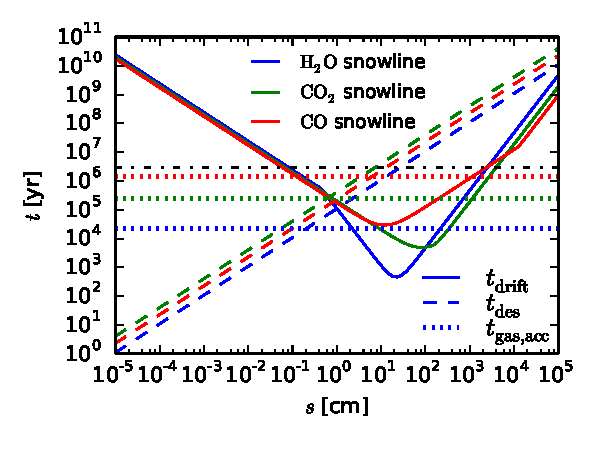
\includegraphics[width=0.5\textwidth]{../../figs/drift_timescales_betaS1_gas_acc_new.pdf}
%\vspace{-0.5in}
\caption{Relevant timescales for dynamical effects in the desorption process: $t_{\rm r, drift}$ (solid lines), $t_{\rm des}$ (dashed lines) and $t_{\rm gas, acc}$ (dotted lines). The timescales are calculated at three representative locations, i.e. the H$_2$O, CO$_2$ and CO snowlines in the static disk. For our choice of parameters, the snowlines are located at $\sim$0.7 AU (blue lines), $\sim$8.6 AU (green lines) and $\sim$59 AU (red lines), respectively. The horizontal dashed line represents a typical disk lifetime of 3 Myr. Radial drift and gas accretion affect desorption in the regions where their respective timescales, i.e. $t_{\rm r, drift}$ and $t_{\rm gas, acc}$, are comparable to the desorption timescale $t_{\rm des}$.} 
\label{fig:timescales}
\end{figure}

%\emgr{Calculate timescale for radial drift following Chiang \& Youdin (2010). Calculate desorption timescale following Hollenbach et al. (2009). Estimate gas accretion timescale for a given $\alpha$. Important: mention that, for simplicity and illustrative purposes, these calculations are performed for a passive disk. Show plot with the timescales as a function of particle size at different snowlines to show the regime in which drift matters}.



\section{Snowline Locations}
\label{sec:snowlines}

\begin{figure*}[tb]
\centering
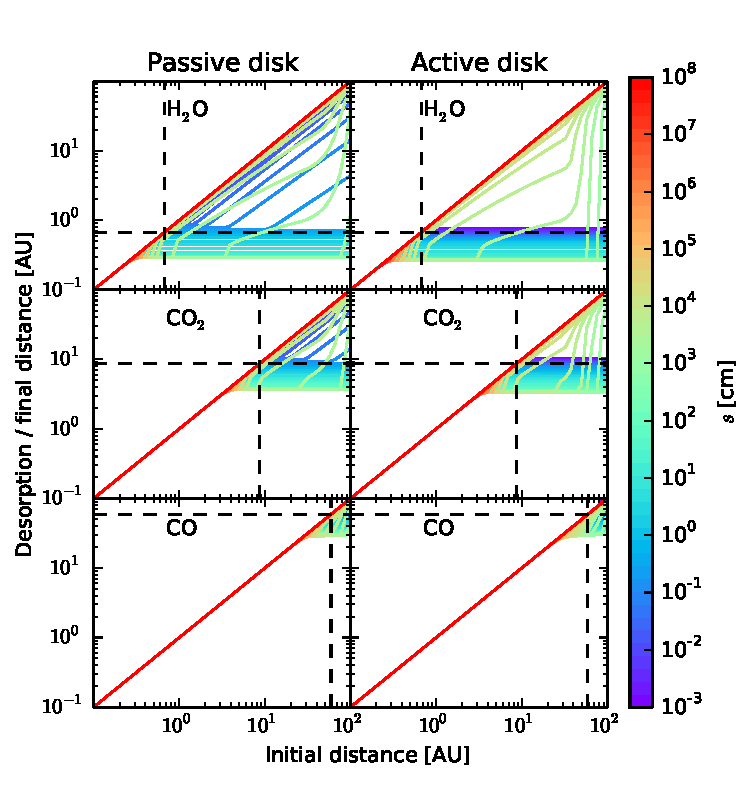
\includegraphics[width=\textwidth]{../../figs/desorption_distance_passive_active_colorbar_test.pdf}
%\vspace{-0.5in}
\caption{Desorption distance as a function of a particle's initial location in the disk, for a range of particle sizes, and for both a passive disk (left panels) and an active disk (right panels). The desorption distance is calculated for particles composed of H$_2$O (top panels), CO$_2$ (middle panels) and CO (bottom panels). The particle size increases from $10^{-3}$ cm to $10^8$ cm as indicated by the color bar. For the range of particle sizes that fully desorb during $t_{\rm d}=3$ Myr, the desorption distance is the same regardless of the particles' initial location.} 
\label{fig:snowlines}
\end{figure*}

\begin{figure*}[t!]
\centering
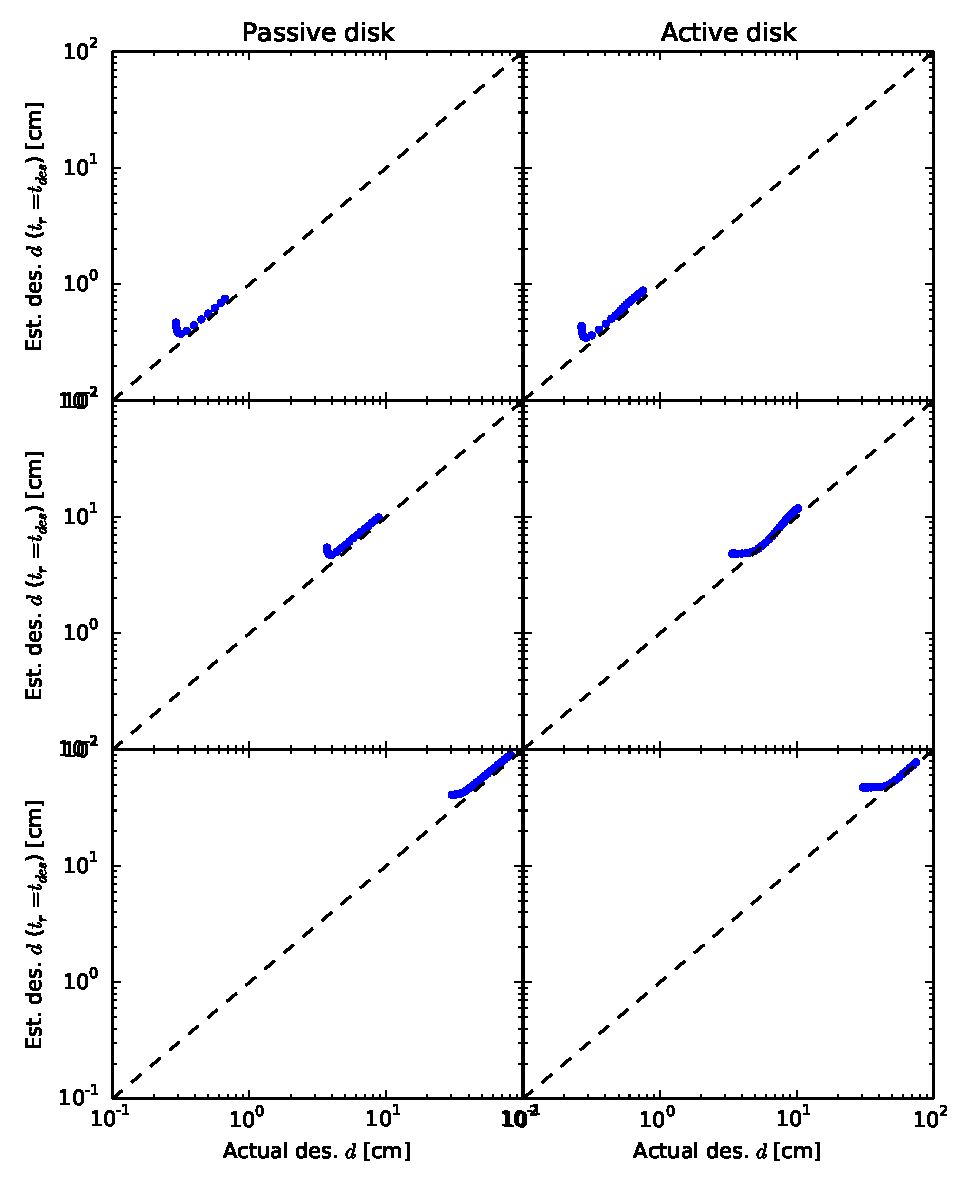
\includegraphics[width=0.7\textwidth]{../../figs/desorption_distance_actual_vs_estimated_passive_active.pdf}
%\vspace{-0.5in}
\caption{Desorption distance estimated from analytic calculations (see text) as a function of the desorption distance calculated numerically, for the range of particle sizes that desorb at a fixed distance regardless of their initial location (see Figure \ref{fig:snowlines} and text). The estimate is performed for a passive disk (left panels) and an active disk (right panels).  The particles are composed of H$_2$O (top panels), CO$_2$ (middle panels) and CO (bottom panels). The analytic approximation is in good agreement with the numerical result for most cases.}
\label{fig:an_vs_actual}
\end{figure*}

In this section we use the model described in section \ref{sec:model} to quantify the effects of radial drift (passive disk) or radial drift and gas accretion (active disk) on the snowline location, for dust particles of different sizes composed of either H$_2$O, CO$_2$ or CO. Specifically, we determine a particle's final location (i.e., where the particle either fully desorbs or remains at its initial size due to a long desorption timescale) as a function of its initial position in the disk, after the gas disk has dissipated. The disk lifetime, $t_{\rm d}$, is particularly relevant since this is the timescale on which giant planets form. The snowline locations at $t=t_{\rm d}$ throughout the protoplanetary disk determine the disk C/O ratio in gas at this time, and thus the C/O ratio in giant planet atmospheres that have formed \textit{in situ}.   



For each species $x$, we determine the final location in the disk of a particle of initial size $s_0$ by solving the following system of coupled differential equations:

\begin{subeqnarray}
\label{eq:ddt}
\frac{ds}{dt} &= & - \frac{3 \mu_x m_{\rm p}}{\rho_{\rm s}} N_x R_{\rm des, x}  \slabel{eq:dsdt} \\
\frac{dr}{dt} &=& \dot{r} \slabel{eq:drdt},
\end{subeqnarray}
where the desorption rate $R_{\rm des, x}$ for each particle type (i.e., composed of H$_2$O, CO$_2$ or CO) is evaluated at $T=T_{\rm d}(r)$, and the radial drift velocity $\dot{r}$ is given by Equation (\ref{eq:rdotpas}) for a passive disk and Equation (\ref{eq:rdotact}) for an active disk. Equations (\ref{eq:dsdt}) and (\ref{eq:drdt}) describe the coupled desorption and radial drift, and can be derived straightforwardly from Equation (\ref{eq:tdes}). Our boundary conditions are $s(t_0)=s_0$, $r(t_0)=r_0$, and $s(t_{\rm d})=0$, where $t_0$ is the initial time at which we start the integration and $r_0$ is the initial location of the particle. We choose $t_0=1$ year, but our result is independent on the initial integration time as long as $t_0 \ll t_{\rm d}$.

As we show in Section \ref{sec:COratio}, a drifting particle that desorbs will do so almost instantaneously and will lose most of its mass very close to the distance at which it fully evaporates. Thus a particle's final location will depend on whether a grain initially at a certain distance is completely desorbed or not within the disk lifetime of 3 Myr. For example, larger grains take longer to desorb and hence are more likely to not evaporate fully in a given timeframe. 

Figure \ref{fig:snowlines} shows our results for H$_2$O, CO$_2$ and CO particles, for both a passive and an active disk. We do not show the equivalent result for the steady-state active disk since the trends are qualitatively the same as for the active disk with the temperature profile given by Equation (\ref{eq:diskT}). Kilometer-sized bodies do not drift or desorb during the disk lifetime neither for a passive nor for an active disk. Similarly, micron- to mm-sized particles in the passive disk do not drift or desorb unless they are located inside the static snowlines. This is not in contradiction with the desorption timescales for small particles from Figure \ref{fig:timescales}, since small grains only desorb fast at or nearby their respective snowlines, as mentioned in Section \ref{sec:timescales}.  In an active disk, however, micron-to mm-sized grains do drift significantly since they move at the same velocity as the accreting gas. For $0.5$ cm $\lesssim s_0 \lesssim$ 700 cm in a passive disk and $0.001$ cm $\lesssim s_0 \lesssim$ 700 cm in an active disk, we notice that particles of initial size $s_0$ desorb at a fixed distance $r_{\rm des}$ regardless of their original location in the disk. In fact, the only grains that will both drift and evaporate are those that reach their fixed final location (represented by the horizontal curves in Figure \ref{fig:snowlines}) within the disk lifetime. We show in section \ref{sec:COratio} that this result is essential in determining the C/O ratio throughout the disk for different particle sizes. 

\begin{figure*}[t!]
\centering
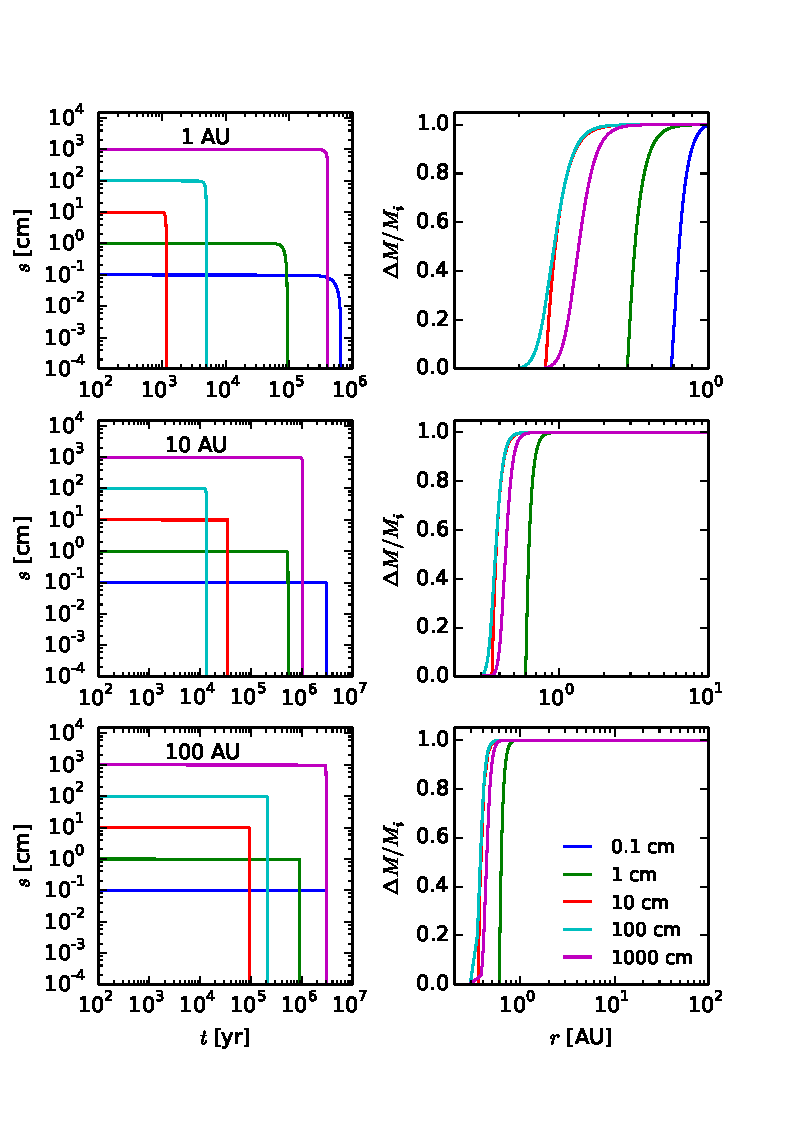
\includegraphics[width=0.8\textwidth]{../../figs/s_t_a.pdf}
%\vspace{-0.5in}
\caption{Left panels: size of desorbing H$_2$O particles as a function of time, for different initial particle sizes and for three initial locations in a passive disk: 1 AU (top left), 10 AU (middle left) and 100 AU (bottom left). Particles desorb almost instantaneously. Right panel: fractional mass of the desorbing particles as a function of the particle's location as it drifts, for different initial particle sizes, and at the same initial locations presented in the left panel. Particles lose most of their mass very close to the distance at which they fully desorb.}
\label{fig:s_t_a}
\end{figure*}


Intuitively, this fixed $r_{\rm des}$ should be the location in the disk for which $t_{\rm r, drift} \sim t_{\rm des}$, given an initial particle size. We can calculate this location analytically by equating Equations (\ref{eq:tdes}) and (\ref{eq:tdrift}) and solving for $r=r_{\rm des}(s)$ for a given particle size $s$. Figure \ref{fig:an_vs_actual} shows $r_{\rm des}$ calculated analytically using the prescription above as a function of the actual desorption distance calculated numerically,  for the range of particle sizes that desorb at a fixed distance in a passive and an active disk (see Figure \ref{fig:snowlines}). We notice that the analytic approximation accurately reproduces the numerical result for most cases of interest, but it slightly deviates for smaller particles. \emgr{I've yet to figure out why there is a discrepancy for the small grains. I'll keep thinking about it, but for now I'll leave it as it is since I don't want to give a false explanation just to have one.} 



%\emgr{I didn't write the text for Figure 4 since we haven't yet decided if in the end we will include it in some form. We can }

%\begin{figure}[h!]
%\centering
%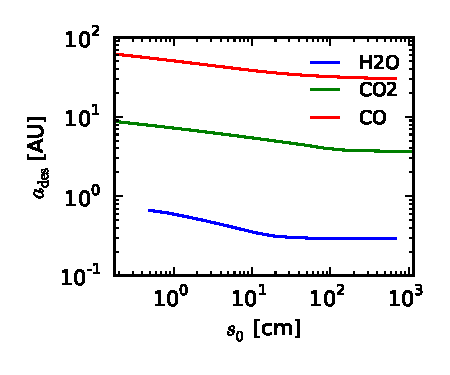
\includegraphics[width=0.5\textwidth]{../../figs/desorption_distance_vs_s.pdf}
%%\vspace{-0.5in}
%\caption{Desorption distance as a function of initial particle size, for the range of particles that desorb at a fixed distance regardless of initial location (see Figure \ref{fig:snowlines}). \textbf{Figure belongs to section 3.} \emgr{This is a figure that I'm not sure we should include, since it doesn't really provide that much useful inside. If we did include it though, there would be two panels both for the passive and the active disk. The caption is not complete since the active disk panel is not yet there.}}  %  (See text for a description of evolution to yet higher masses.) 
%\label{fig:r_vs_s}
%\end{figure}

%\emgr{Present the equation set that you are solving, $dr/dt=\dot{r}$, $ds/dt=...$. I don't think it is necessary to describe in detail the numerical method of solving the equations since it's pretty straightforward. Present the pretty rainbow plots side by side for passive and active disks, and highlight the differences. Insert the plots that shows that for the intermediate size particles, the desorption distance can be estimated analytically with good accuracy. Maybe also include the plot showing the desorption distance as a function of particle size, both for passive and active disk. Split into subsections?}


\section{Results for the C/O Ratio}
\label{sec:COratio}


We now use our model and the results of Section \ref{sec:snowlines} to determine the H$_2$O, CO$_2$ and CO snowline locations and the C/O ratio in disks with static chemistry that experience radial drift of solids and gas accretion on to the central star. In Section \ref{sec:snowlines}, we showed that solid particles that drift and fully desorb during the lifetime of the protoplanetary disk do so (1) instantaneously, and (2) at a fixed stellocentric distance, regardless of their initial location in the disk. Figure \ref{fig:s_t_a} confirms both of these effects. The left panels show the size evolution with time for H$_2$O particles of various initial sizes, starting at three different initial locations in a passive disk \footnote{Our conclusions remain valid for an active disk and for particles composed of CO$_2$ or CO.}.  Indeed, the solid H$_2$O particles evaporate almost instantly, although the time $t_{\rm des}$ at which a particle of a given initial size desorbs depends on its initial distance. A particle located at the initial time $t_0$ at a distance such that $t_{\rm des}>t_{\rm d}$ will therefore not desorb during the disk lifetime. However, our model assumes that particles drift continuously at any location in the disk. Therefore, a particle that can fully desorb during the disk lifetime for at least one initial location will always desorb, at a fixed distance as discussed in Section \ref{sec:snowlines} and displayed in Figure \ref{fig:snowlines}. The right panels of Figure \ref{fig:s_t_a} show that the drifting grains lose most of their mass in a very narrow distance range; moreover, this distance is the same for a given initial particle size, no matter where the particle started drifting at the time $t_0$ when the simulation is started. Figure \ref{fig:s_t_a} thus proves claims (1) and (2) above. It follows that the H$_2$O, CO$_2$ and CO snowlines are fixed for a given initial particle size and disk model (passive or active). The C/O ratio will then only depend on disk properties, grain size, and the abundance of H$_2$O, CO$_2$ and CO relative to the H$_2$ abundance in the disk midplane. 

\begin{figure}[h!]
\centering
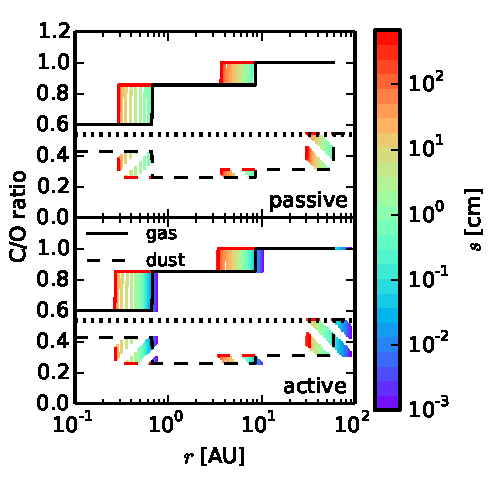
\includegraphics[width=0.5\textwidth]{../../figs/C_O_ratio_passive_active_disk_many_colorbar_test.pdf}
%\vspace{-0.5in}
\caption{C/O ratio in gas (solid lines) and in dust (dashed lines) for a passive disk (top panel) and for an active disk (bottom panel), and for the range of particle sizes that desorb at a fixed distance regardless of their initial location in the disk. The particle size increases from 0.001 cm to $\sim$700 cm as indicated by the color bar. The horizontal dotted line represents the stellar value of 0.54. The black lines represent the C/O ratio in gas (solid black line) and dust (dashed black line) for a static disk. The snowline location moves inward as the particle size increases. \emgr{Some additional text for the currently non-existent third panel.}}
\label{fig:CO_ratio}
\end{figure}

We use the relative number densities of C and O in their different molecular forms (H$_2$O, CO$_2$ and CO) from Table 1 of \citet{oberg11}. \emgr{Is it necessary to reproduce that table? Seems a bit redundant.}. Figure \ref{fig:CO_ratio} shows the C/O ratio in gas and dust as a function of semimajor axis for a passive disk, an active disk with a passive temperature profile, and a steady-state active disk \emgr{(not yet there)}. The C/O ratio for a static disk is shown as a guideline. The plot is consistent with Figure \ref{fig:snowlines}. For the passive disk, only grains larger than $\sim$0.5 cm drift, desorb and thus form a snowline. In contrast, even $\sim$micron-sized grains drift and desorb for the active disk, since they flow towards the host star together with the accreting gas. For the same particle size, the snowline locations are slightly closer to the central star in the active disk, due to the fact that the accreting gas adds an additional component to the drift velocity of the solids (cf. Equation \ref{eq:rdotact}). Perhaps the most interesting feature is the fact that the snowlines are pushed inwards as the grain size increases. While the plot only shows the snowlines and C/O ratio for particle sizes up to $\sim$7 m, we have found that almost kilometer-sized boulders are able to drift and desorb for both the passive and the active disk. However, bodies larger than $\sim$7 m will evaporate at the same location as the meter-sized planetesimals. Thus the innermost snowlines (depicted in red in Figure \ref{fig:CO_ratio}) set the limit on how close in the H$_2$O, CO$_2$ and CO snowlines can be pushed due to radial drift and gas accretion on to the host star. Realistic grain size distributions in disks are dominated by large grains (e.g., \citealt{dalessio01}, \citealt{birnstiel12}). Therefore, the snowlines produced by the largest drifting solids in our model set the inner limit on the snowline locations and are insensitive to a particular grain size distribution. \emgr{There will be 1-2 additional sentences for the third panel, the steady-state disk, once that finishes running.}





%\begin{figure}[h!]
%\centering
%\includegraphics[width=0.5\textwidth]{lala}
%%\vspace{-0.5in}
%\caption{C/O ratios for different particle size distributions... \textbf{Figure belongs to section 4.} (\emgr{It will probably be a multi-panel plot, for different particle size distributions, for both passive and active disk, and perhaps at different times for the active disk. Not yet unsure how that figure will look like since I don't have the results yet, so I'll leave the figure caption open for now.})}
%\label{fig:...}
%\end{figure}

%\emgr{Motivate the fact that we can calculate a sharp, fixed snowline for each particle size by inserting the plot that shows that particles desorb almost instantaneously at a fixed distance.  Then present the plots analogous to Fig. 1 in \"Oberg et al. (2011) for different particle sizes, based on the snowline locations obtained in the previous section, both for passive and active disk. Perhaps show it at different times in the gas disk evolution (i.e., not just at 3 Myr) for the active disk. Then assume a particle size distribution and show the interpolated result for the C/O ratio. Generalize the result using a transition disk (this part might also fit in the discussion section).}

%emgr{Present the flux equations used to keep track of the amount of C and O in gas and dust throughout the disk. Motivate the simplification of using a fixed particle sized, fixed timescale, and fixed desorption distance in the calculations by referring to the rainbow plot in the previous section and by inserting the plot that shows that particle desorb almost instantly at a fixed distance. Based on these assumptions, finally show the equivalent of Fig. 1 in \"Oberg et al. (2011) for different particle sizes, and at different times in the gas disk evolution (i.e., not just at 3 Myr) --- a multi-panel plot could be a good idea. Discuss the result, trends, etc. Ideally, have a final plot showing the results for a particle size distribution rather than for individual particles.}

\section{Discussion and Model Limitations}
\label{sec:discussion}

\begin{figure*}[t!]
\centering
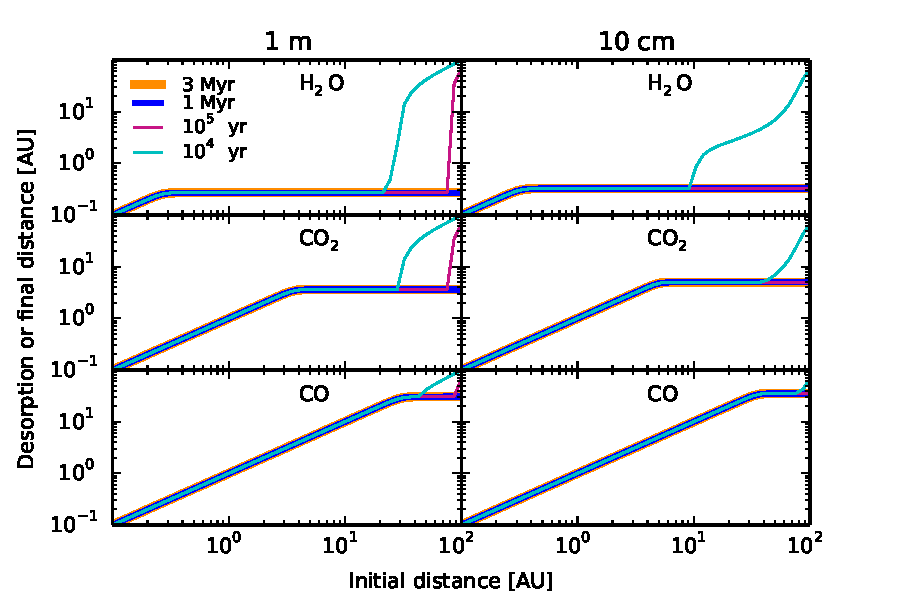
\includegraphics[width=\textwidth]{../../figs/time_plots.pdf}
%\vspace{-0.5in}
\caption{Desorption / final distance as a function of initial position in the disk for particles of initial size $s_0=1$ m (left panels) and $s_0=10$ cm (right panels), for grains composed of H$_2$O (top panels), CO$_2$ (middle panels) and CO (bottom panels). The evolution is shown at four representative timescales: $10^4$ yr (cyan curve), $10^5$ yr (red curve), 1 Myr (green curve), and 3 Myr, the disk lifetime (blue curve). For a given particle size, the desorption distance, and hence the H$_2$O, CO$_2$ and CO snowlines, have the same location regardless of the time at which the simulation is stopped.}
\label{fig:timeplots}
\end{figure*}

\begin{figure}[h!]
\centering
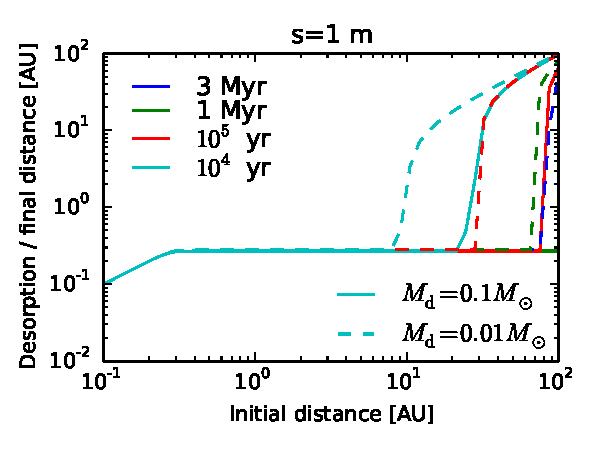
\includegraphics[width=0.5\textwidth]{../../figs/desorption_distance_varying_Md.pdf}
%\vspace{-0.5in}
\caption{Desorption / final distance as a function of initial position in the disk for H$_2$O particles of initial size of 1 m, for total disk masses $M_{\rm d}=0.1 M_{\odot}$ (solid lines) and $M_{\rm d}=0.01 M_{\odot}$ (dashed lines). The timescales of the simulations and their color code are the same as in Figure \ref{fig:timeplots}. A lower disk mass does not change the snowline location.}
\label{fig:varMd}
\end{figure}

\subsection{Generality of Results: Dependence on Disk Parameters}
\label{sec:incond}

In this section we investigate how variations in our fiducial parameters, such as the total disk mass or the time in the disk evolution at which we determine the snowline locations and the C/O ratio, affect our results. The disk lifetime $t_{\rm d}=3$ Myr is the most representative for our calculations, as this is the timeframe in which giant planets accrete their gaseous atmospheres (e.g., \citealt{pollack96}, \citealt{piso14}). However, protoplanetary cores start acquiring their envelope at earlier times, before the core is fully formed (e.g., \citealt{rafikov06}). Recent models such as aerodynamic pebble accretion \citep{lambrechts12} suggest rapid core growth on timescales of $10^5$ years, which implies that the time when cores accrete their massive envelope may be at least an order of magnitude shorter than the disk lifetime. The composition of giant planet atmospheres, and specifically their C/O ratio, can thus depend on the abundance of H$_2$O, CO$_2$ and CO in gas and dust forms at earlier times than $t_{\rm d}$ in the disk evolution. 

Figure \ref{fig:timeplots} shows the desorption or final distance as a function of a particle's initial location in the disk, for grains of initial sizes of 10 cm and 1 m, composed of either H$_2$O, CO$_2$ or CO. These sizes are representative since radial drift timescales are shortest for particles within this size range (see Figure \ref{fig:timescales}) --- these are the particles whose drift and desorption evolution should be most strongly affected by variations in disk conditions. We perform the simulations at four representative timescales in the disk evolution to see how the snowline locations evolve with time and affect the C/O ratio. Particles that start at large stellocentric distances do not desorb within the shorter timeframes, e.g. $10^4$ or $10^5$ years. However, they do evaporate if their initial location is closer to the host star. As stated in Section \ref{sec:COratio}, this implies that the grains form a snowline even after $10^4$ years. More importantly, for a given initial grain size, the snowline locations are independent of the time elapsed. Therefore, our results are not only valid at $t_{\rm d}$, but also throughout the earlier time evolution of the protoplanetary disk. 

We choose as a fiducial model a total disk mass $M_{\rm d}=0.1 M_{\odot}$, but this number is not universally valid. From observations of the dust continuum, \citet{andrews13} find that a linear scaling $M_{\rm d} \propto M_*$ is reasonable. Giant planets, however, have been detected around small stars (e.g., \citealt{montet14}), which can have masses as low as $M_* \sim 0.1 M_{\odot}$. We thus explore the effect of disk mass on the location of snowlines. Figure \ref{fig:varMd} shows the desorption or final distance as a function on the initial location of a H$_2$O particle with initial size of 1 m, for two total disk masses: $M_{\rm d}=0.1 M_{\odot}$, our fiducial model, and $M_{\rm d}=0.01 M_{\odot}$. The simulations are stopped after the same timeframes as those in Figure \ref{fig:timeplots}. The location of the H$_2$O snowline is the same for both disks (the same holds true for the CO$_2$ and CO snowlines). The C/O ratio is thus insensitive to the choice of $M_{\rm d}$. This result also has implications for transition disks, which have inner cavities significantly depleted of dust (e.g., \citealt{espaillat12}). Since the snowline locations are independent of disk mass, we expect transition disks to exhibit the same drift-desorption behavior as standard disks under the simplified assumptions of our model.     



\subsection{Neglected Effects}
\label{sec:neglected}

Our goals in this paper were (1) to gain a detailed qualitative and quantitative understanding of the effect of radial drift and gas accretion on to the central star on snowline locations and the C/O ratio in disks, and (2) to obtain a limit on how close in the snowlines can be pushed due to drift and gas accretion. We have thus used a simplified model and out of necessity neglected potentially significant dynamical and chemical processes. In what follows, we discuss these limitations and their effects. We note that our future work will address some of these issues. 

\begin{table}[t!]
\caption{Dynamical and chemical processes that affect the snowline locations of the main C and O carriers, H$_2$O, CO$_2$ and CO. The arrows signify the direction in which a particular process affects the snowlines: $\leftarrow$ means that the snowline is pushed closer to the host star, $\rightarrow$ means that the snowline is pushed further from the host star. The presence of both arrows means that the process may have both effects on the snowline location.}
\begin{center}
\begin{tabular}{|l|l|}\hline
\textbf{Process} & \textbf{Effect} \\\hline
Radial drift & $\leftarrow$ \\\hline
Gas accretion & $\leftarrow$ \\\hline
Particle growth & $\rightarrow$ \\\hline
Turbulent diffusion & $\rightarrow$ \\\hline
Particle fragmentation & $\rightarrow$ $\leftarrow$ \\\hline
Morphology & $\rightarrow$ \\\hline
Particle composition & $\rightarrow$ $\leftarrow$ \\\hline
Non-static chemistry & $\rightarrow$ $\leftarrow$ \\\hline
\end{tabular}
\end{center}
\end{table}

We summarize in Table 1 the potential physical and chemical processes occurring in disks and their effect on snowline locations. For the sake of completion, Table 1 also includes the processes addressed in this paper, i.e. radial drift and gas accretion. The neglected effects are discussed in more detail below. 



\begin{enumerate}
\item \textbf{Particle growth.} While our model assumes a range of particle sizes, each size is considered fixed for a given grain throughout its drift and evolution. However, grain growth has been observed in protoplanetary disks (e.g., \citealt{ricci10}, \citealt{perez12}), as well as theoretically constrained (e.g., \citealt{birnstiel10}, \citealt{birnstiel12}). In Section \ref{sec:COratio} we have shown that larger grains move the snowline locations closer in, but those locations remain fixed above a certain particle size. Once the solids grow larger than km-sized, they are no longer affected by drift or desorption, and the snowline reduces to that of a static disk. It follows that grain growth will eventually push the snowline location outwards.

\item \textbf{Turbulent diffusion.} The radial drift model presented in Section \ref{sec:drift} only considers a laminar flow and thus ignores turbulence. However, the disk gas also experiences turbulent diffusion (e.g., \citealt{birnstiel12}, \citealt{alidib14}). Turbulence causes eddies and vertical mixing, which are likely to reduce the radial gas accretion velocity. Additionally, the flow of H$_2$O, CO$_2$ and CO vapor will diffuse radially, causing it to cross the snowline and refreeze, thus moving the snowline location outwards altogether.

\item \textbf{Particle fragmentation.} Frequent particle collisions in disks cause them to fragment (e.g., \citealt{birnstiel12}). The fragmentation of meter- to km-sized particles will move the snowlines outwards, as smaller particles desorb faster and further out from the host star (cf. Figures \ref{fig:snowlines} and \ref{fig:CO_ratio}). Large boulders, which neither drift nor desorb, may become e.g. meter-sized due to collisions and subsequent fragmentation, which will cause them to drift significantly before desorbing, pushing the snowlines inwards. Thus fragmentation can move the snowline locations in either radial direction.

\item \textbf{Morphology.} Our model assumes that the ice particles are perfect, homogeneous spheres. However, this is not a very good approximation, since grain growth can be fractal rather than compact (\citealt{zsom10}, \citealt{okuzumi12}). The inhomogeneity due to cracks in the grain structure will cause the particles to desorb faster. They will therefore drift less before evaporating and will move the snowlines outwards.

\item \textbf{Particle composition.} The ice particles in our model are assumed to be fully formed of either H$_2$O, CO$_2$ or CO. In reality, the grains have a layered structure, such as an interior composed of non-volatile materials (e.g., sillicates) covered by an icy layer. The ice thus only constitutes a fraction of the total particle mass, which accelerates its desorption and pushes the snowlines outwards. The grains may also be composed of a mixture of H$_2$O, CO$_2$ and CO ices. The relative fraction of each volatile, as well as their degree of mixing, will determine their desorption timescale, and as a result whether the snowlines are moved towards or away from the central star.

\item \textbf{Non-static chemistry.} As the goal of this paper was to explore only the dynamical effects on snowline locations and the C/O ratio in disks, we have assumed a simple, static chemical model. However, gas-grain chemistry is very complex and time-dependent. In the inner disk, chemistry approaches equilibrium due to intense sources of ionizing radiation (e.g., \citealt{ilgner04}), while in the outer disk high energy radiation and cosmic rays are the key drivers of chemistry, which is no longer in equilibrium (e.g., \citealt{vandishoeck06}). A multitude of chemical evolution models have been developed (see references in \citealt{henning13}), many of which contain tens or hundreds of chemical reactions. Due to the complexity of these chemical models, most of them are decoupled from disk dynamics. The effect of disk chemistry on snowline locations, shape, time evolution, or the C/O ratio is therefore difficult to estimate.  In a future paper, we plan to parametrize the chemical model developed by Merchantz et al. (in preparation) that traces the evolution of the main C and O oxygen carriers, and incorporate it in our radial drift calculation. 

\end{enumerate}



%\emgr{Present the diagram that shows all the effects that can modify snowline location. For model limitations, include: non-inclusion of turbulence, assumption of perfect spheres when in fact they may have cracks, particles composed of a single volatile when in reality they are likely to be mixed, etc. Discuss uncertainty of initial conditions and estimate how much they matter. ....}

\section{Summary}

\emgr{To be done soon.}

%\appendix
%\section{...}
%
%\emgr{Right now it's unclear to me what could go in an appendix, if anything. Maybe discuss a bit the algorithm to evolve $\Sigma_{\rm p}$ (although it is already explained in detail in the appendix of Birnstiel et al. 2010). Maybe show some example profiles of $\Sigma_{\rm p}$ at different times and for different particle sizes.}

\if\bibinc n
\bibliography{refs}
\fi

\if\bibinc y
\begin{thebibliography}
\end{thebibliography}
\fi


\end{document}